\rhschapter{Implementering}
I følgende afsnit vil der blive gennemgået hvordan spillets logik er implementeret i Unreal Engine 4.

\section{Menu}
\textit{Af Mathias Forsberg}\newline
Menuen er lavet i et Widget Blueprint hvori der er sat knapper op i en vertical box. Knapperne har tilhørende tekst som indikere deres funktion. Derudover er der sat et PNG-billede ind som baggrund for menuen. Play-knappen har et OnClick event der sørger for at skifte scene til gamemoden når der bliver trykket på den. Quit-knappen bruger en "Execute Console Command" til at lukke spillet ned nåt der bliver trykket på knappen. Se figur \ref{dia:menublueprint}. Menu blueprintet ligger inde i sin egen level, hvor den er instansieret i viewporten.

\begin{figure}
	\begin{center}
		\caption{Menuens blueprint.}
		\label{dia:menublueprint}
		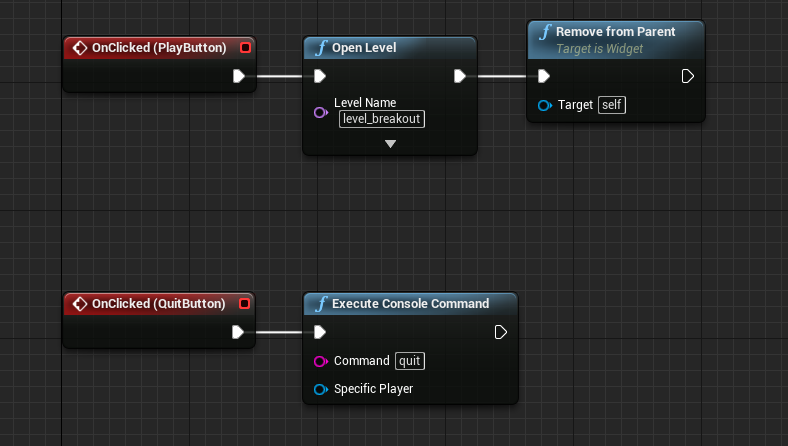
\includegraphics[width=0.80\linewidth]{pictures/blueprints/menu_blueprint}
	\end{center}
\end{figure}

\section{Level}
\textit{Af Nichlas Bruun}\newline
Level blueprintet er banens "klasse". Denne har ikke meget, og forholdvist simpel logik. Når banen, eller selve spillet startes, bliver \textit{EventBeginPlay} kaldt, hvilket betyder at logikken der ligger i dette event kun bliver kaldt en gang når der startes med at spille. På dette event ligger logikken til at skifte synspunktet til kameraet i selve spilbanen, og logikken til at binde UI-blueprintet til samme viewport. Se figur \ref{dia:levelblueprint}.

\begin{figure}
	\begin{center}
		\caption{Banens blueprint.}
		\label{dia:levelblueprint}
		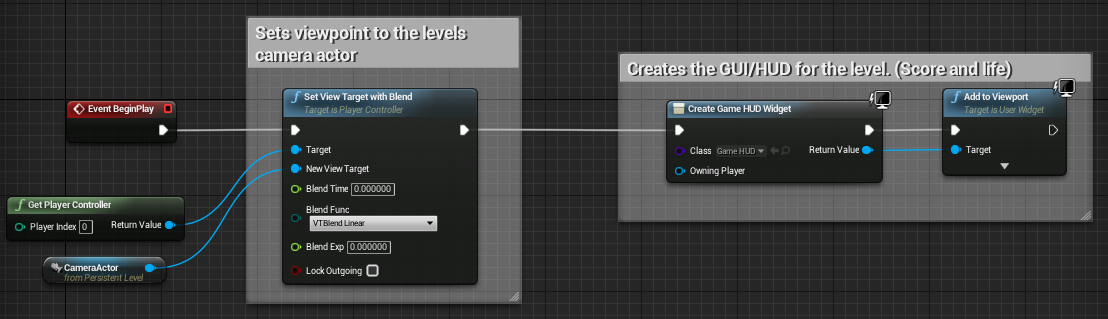
\includegraphics[width=0.98\linewidth]{pictures/blueprints/level_blueprint}
	\end{center}
\end{figure}

\section{UI}
\textit{Af Bjarne Kristensen}\newline
GameHUD blueprint er et Widget Blueprint der viser UI mens man spiller. Den indeholder blot fire tekst felter, hvor to af dem er teksterne; "Balls" og "Score". De to andre tekst felter bliver opdateret løbende, med liv og score, når man spiller spillet. Se figur \ref{dia:gamehuddesign} for designet.

\begin{figure}
	\begin{center}
		\caption{Spillets HUD(Heads Up Display).}
		\label{dia:gamehuddesign}
		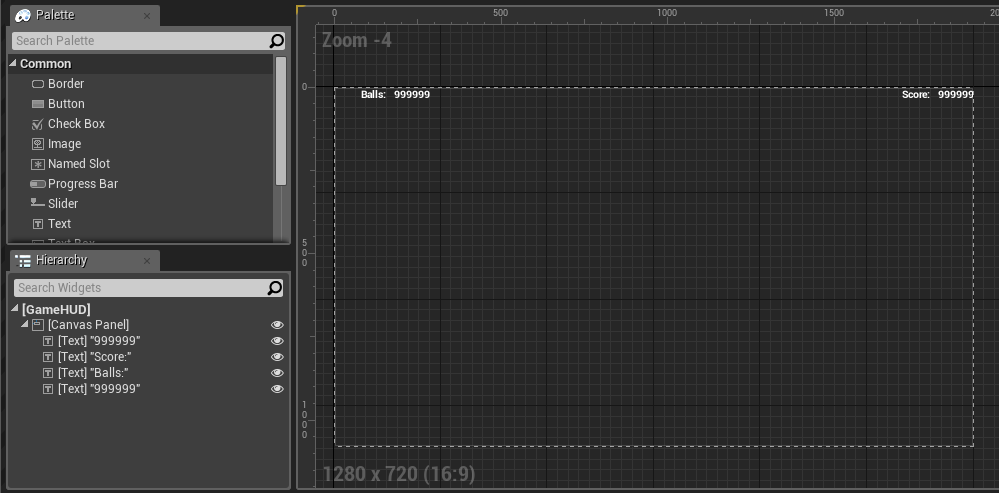
\includegraphics[width=0.98\linewidth]{pictures/blueprints/gamehud-design}
	\end{center}
\end{figure}

Der er to funktioner i GameHUD blueprintet; Balls og Score. Det er disse to funktioner som holder tekst felterne opdateret. Balls og Score variablerne er sat i Paddle Blueprint instansen på Paddle objektet i selve banen. For at få fat i disse variabler fra en anden instans, er man nødt til at søge efter instansen og så gemme en pointer til instansen lokalt hvor man skal bruge den. Da der kun er en paddle i banen kan vi bare tage den første instans der findes og sætte den i vores lokale variabel. Efter paddle blueprint instansen er fundet kan f.eks. Score variablen konverteres til tekst og returneres til GameHUD blueprintet hvor teksten så bliver opdateret. Se figur \ref{dia:gamehudscorefunction}. Tilsvarende sker med Balls variablen i en funktion som opdaterer teksten med hvor mange liv man har tilbage.

\begin{figure}
	\begin{center}
		\caption{GameHUD opdater Score tekst funktion.}
		\label{dia:gamehudscorefunction}
		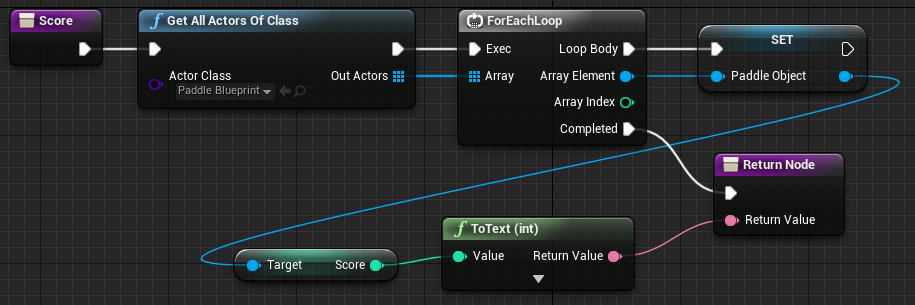
\includegraphics[width=0.98\linewidth]{pictures/blueprints/gamehud-score-function}
	\end{center}
\end{figure}

\section{Paddle}
\textit{Af Mathias Forsberg, Bjarne Kristensen og Nichlas Bruun}\newline
Paddlen er inddelt i højre og venstre halvdel, dette er gjort ved lave et tjek på hvor bolden rammer paddlen. Hvis boldens X-værdi når den rammer paddlen er mindre end placeringen af paddlens midte, har bolden ramt venstre side og er X-værdie derimod større end placeringen af paddlens midte, har den ramt højre. Hele dette tjek bruges til at give bolden den rette udgangsvinkel efter kollisionen med paddlen er sket. Herefter bliver der lavet et tjek på hvor boldens tidligere placering var, hvilket bruges til at udregne hvilken retning bolden kommer fra. Et eksempel på dette kan være hvis bolden kommer fra højre side i forhold til paddlens placering og rammer højre side af paddlen vil bolden flyve tilbage i den retning den kom fra, ved at vende fortegn i begge af boldens akser.

Paddlen modtager også input fra tastaturet for at kunne bevæge den fra side til side. Man skal først aktivere input på \textit{player controlleren} for at kunne behandle input. Se figur \ref{dia:paddleenableinput}. 

\begin{figure}
	\begin{center}
		\caption{Blueprint: Aktivere input.}
		\label{dia:paddleenableinput}
		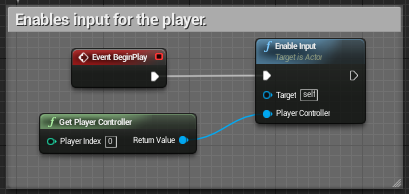
\includegraphics[width=0.60\linewidth]{pictures/blueprints/paddle-enable-input}
		\end{center}
\end{figure}

Når man trykker på enten A eller ventre pil tasterne, sætter vi en boolean variabel \textit{IsAPressed} til true. Når spilleren så slipper tasterne igen, bliver den sat til false. Denne bliver brugt til at rykke paddlen mod ventre i banen. Se figur \ref{dia:paddlehandleinput}. Fremover bliver der refereret til A selvom det også kan være pil venstre der er trykket ned. Det er det same der bliver gjort mod højre retning med \textit{IsDPressed}. Hvis man trykker på escape tasten loader den banen der har hoved menuen. Trykker man på space tasten bliver \textit{IsSpacePressed} sat til true, og false når man slipper tasten.

\begin{figure}
	\begin{center}
		\caption{Blueprint: Håndtere input.}
		\label{dia:paddlehandleinput}
		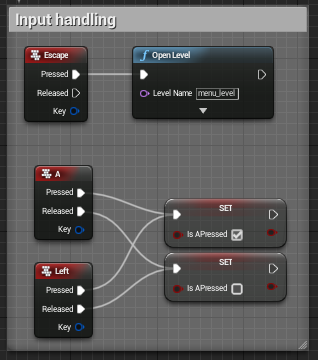
\includegraphics[width=0.50\linewidth]{pictures/blueprints/paddle-handle-input}
		\end{center}
\end{figure}

Det første der sker i EventTick'et er at vi ser om der bliver trykket på space. Dette sætter en anden variabel så bolden kan blive skudt afsted. Hvis man ikke trykker på space og bolden ikke er skudt afsted så den flyver frit rundt, skal den låses fast lige oven over paddle'en. Se figur \ref{dia:paddlelockball}.

\begin{figure}
	\begin{center}
		\caption{Blueprint: Sæt til at skyde eller få bolden til at følge battet hvis den ikke er skudt.}
		\label{dia:paddlelockball}
		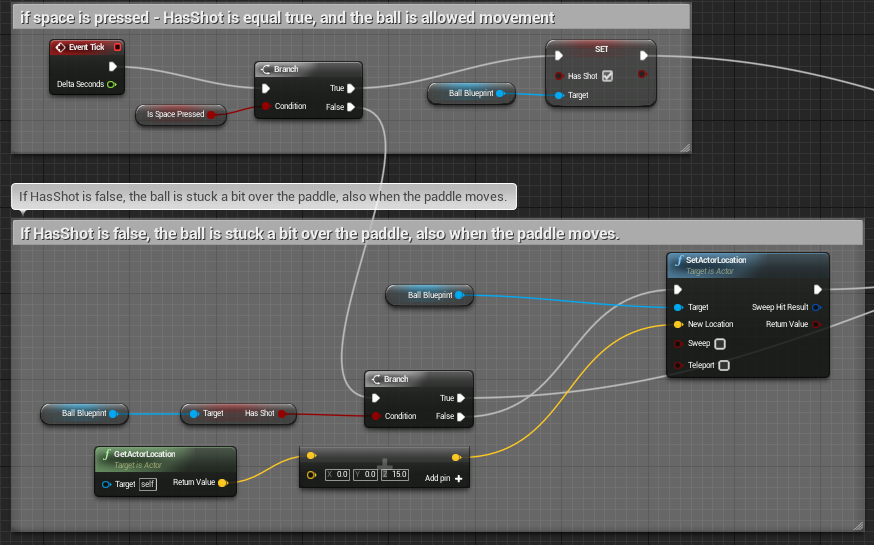
\includegraphics[width=0.98\linewidth]{pictures/blueprints/paddle-lock-ball}
		\end{center}
\end{figure}

Efter det kontrolleres der om A er trykket ned, men ikke A og D på samme tid. Hvis begge er trykket ned har vi ikke lyst til at den skal bevæge sig mod venstre. Se figur \ref{dia:paddleisapressed}.

\begin{figure}
	\begin{center}
		\caption{Blueprint: Kun aktivere hvis kun A er trykket og ikke A og B på samme tid.}
		\label{dia:paddleisapressed}
		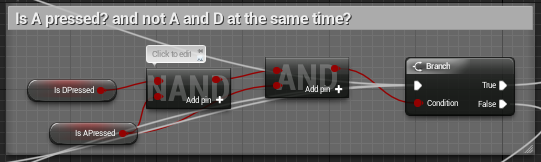
\includegraphics[width=0.80\linewidth]{pictures/blueprints/paddle-is-a-pressed}
		\end{center}
\end{figure}

Hvis kun A er trykket kan vi bevæge paddle'en mod venstre med en given hastighed. For at den ikke skal flytte sig ud over banens sider, er der sat en minimum X værdi som den skal være over for at kunne flytte sig mod venstre. Se figur \ref{dia:paddlemoveleft}. 

\begin{figure}
	\begin{center}
		\caption{Blueprint: Flytter sig mod venstre hvis over minimums grænsen.}
		\label{dia:paddlemoveleft}
		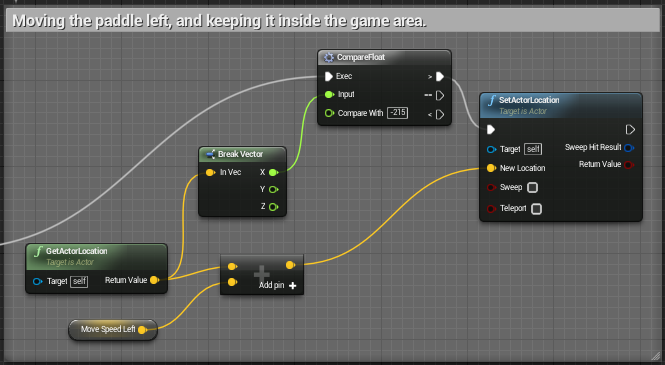
\includegraphics[width=0.98\linewidth]{pictures/blueprints/paddle-move-left}
		\end{center}
\end{figure}

Noget lignende funktionalitet gør sig gældende for at bevæge sig mod højre, bare med modsatte værdier for når D er trykket ned, men ikke D og A på samme tid.

\section{Ball}
\textit{Af Mathias Forsberg og Nichlas Bruun}\newline
Hvis bolden ikke er blevet skudt af fra paddlen vil den være låst fast til paddlen. Derimod hvis den er skudt fra paddlen vil bolden rykke sig med den hastighed der er sat af den lokale variabel \textit{direction vector}. Direction vector variablen bliver ændret alt efter hvad bolden kollidere med. Som tidligere nævnt i paddle afsnittet ligger logikken til kollision med paddlen i paddle blueprintet, derfor er der et tjek på om bolden kollidere med paddlen. Kollidere bolden ikke med paddlen bliver der tjekket på hit eventets \textit{hit normal variabel}, denne værdi fortæller hvilken side af bolden kollidere. Dette kan f.eks. være hvis \textit{hit normal X} er minus 1 er der tale om at boldens venstre side kollidere med et andet objekt. Gennem alle disse tjek kan der udregnes hvilket fortegn i hvilken akse der skal vendes i direction vectoren for at bolden får den korrekte retning efter kollision. I selve bold blueprintet ligger der også tjek på om spilleren har flere liv tilbage, eller om alle brikker er forsvundet fra spilverdenen. Dette sørger for at spilleren kommer tilbage til menuen hvis alle liv er mistet og at der bliver skabt nye brikker hvis alle brikkerne er ramt af bolden. Blueprintet indeholder også et tjek på om bolden er indenfor banen, befinder bolden sig ikke på banene mere vil der blive trukket 1 fra spillerens liv. Sidst men ikke mindst ligger der også logik for inputtet til at skyde bolden fra paddlen, dette gøres ved at når der trykkes på mellemrumstasten sættes den boolske værdi i \textit{has shot} variablen til true, og bolden går igennem det tidligere nævnte tjek.  

\section{Brick}
\textit{Af Nichlas Bruun}\newline
Brick er et blueprint som nedarver fra \textit{PaperSpriteActor}-blueprinttypen, dette vil sige at det er et blueprint der kan instansieres i verdenen med en sprite. Som sådan er det også den eneste logik der ligger på brick, årsagen til at den har et blueprint er for at Ball klassen kan kende forskel på hvad den rammer på \textit{OnHit}-events. Da det ikke ville være hensigten at fjerne f.eks. væggen i siden af banen når den blev ramt af bolden.

